\documentclass{standalone}   % produces a single-page PDF with just the figure
\usepackage{tikz}
\usetikzlibrary{shapes.geometric, arrows, positioning}

\begin{document}
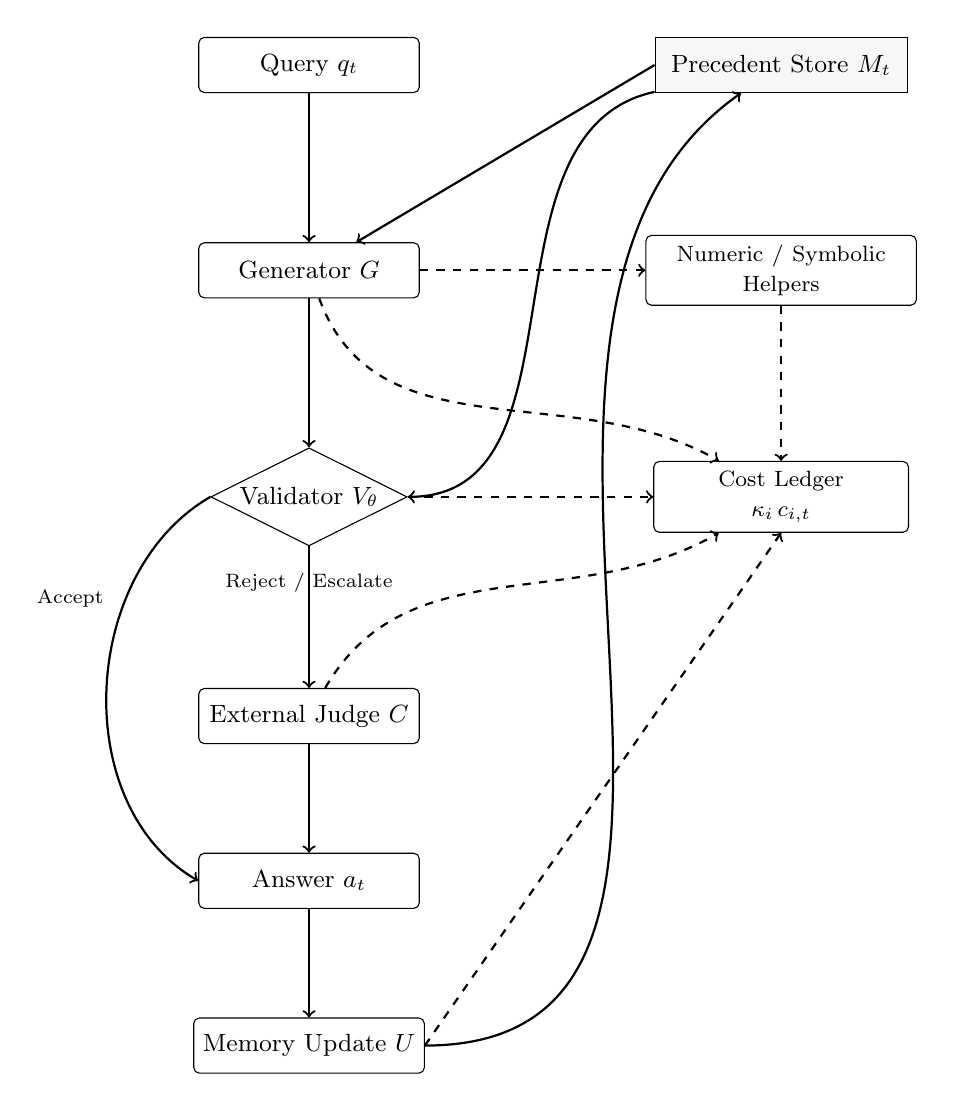
\begin{tikzpicture}[
    node distance = 18mm and 28mm,          % <-- more space
    every node/.style = {font=\small},
    process/.style   = {rectangle, draw, rounded corners=2pt,
                        minimum width=28mm, minimum height=7mm},
    datastore/.style = {rectangle, draw, fill=black!3,
                        minimum width=32mm, minimum height=7mm},
    decision/.style  = {diamond, aspect=2, draw, inner sep=1pt},
    dashedarrow/.style = {->, dashed, thick},
    solidarrow/.style  = {->, thick}
  ]
  
  \matrix[row sep=18mm,column sep=28mm]{
    % row 1
    \node[process]   (query)  {Query $q_t$}; &
    \node[datastore] (memory) {Precedent Store $M_t$}; \\
    % row 2
    \node[process]   (generator) {Generator $G$}; &
    \node[process,text width=32mm,align=center] (helper)
         {\footnotesize Numeric / Symbolic\\Helpers}; \\
    % row 3
    \node[decision]  (validator) {Validator $V_\theta$}; &
    \node[process,text width=30mm,align=center] (ledger)
         {\footnotesize Cost Ledger\\$\kappa_i\,c_{i,t}$}; \\
    % row 4
    \node[process] (judge) {External Judge $C$}; &
    \\[-1.2em] % tighten empty right cell
    % row 5
    \node[process] (answer) {Answer $a_t$}; &
    \\[-1.2em]
    % row 6
    \node[process] (update) {Memory Update $U$}; &
    \\
  };
  
  
  % arrows (identical to previous code)
  \draw[solidarrow] (query) -- (generator);
  \draw[solidarrow] (memory.west) -- (generator);
  \draw[dashedarrow] (generator) -- (helper);
  \draw[dashedarrow] (helper) -- (ledger);
  \draw[solidarrow] (generator) -- (validator);
  \draw[solidarrow]
      (validator.west)      % 1️⃣ step left 7 mm
      to[out=-150,in=150]
      node[pos=.3,left=0.15]{\scriptsize Accept}
      (answer.west);                    % 3️⃣ land on Answer
  \draw[solidarrow] (validator) -- node[pos=.4,above]{\scriptsize Reject / Escalate} (judge);
  \draw[solidarrow] (judge) -- (answer);
  \draw[solidarrow] (memory) to[out=-168,in=0] (validator);
  \draw[solidarrow] (answer) -- (update);
  \draw[solidarrow] (update) to[out=0,in=215] (memory);
  \draw[dashedarrow] (update.east) -- (ledger.south);
  \draw[dashedarrow] (generator) to[out=-70,in=150] (ledger);
  \draw[dashedarrow] (judge) to[out=60,in=-150] (ledger);

  \foreach \n in {validator}
    \draw[dashedarrow] (\n.east) -- (ledger.west);
  
  \end{tikzpicture}
\end{document}  
